\paragraph{}
Au niveau de la prise de sons, il y a la possibilité d'améliorer celle ci et obtenir plus de précision 
en implémentant un algorithme permettant de détecter quels sont les seuils à prendre en compte pour la prise de son 
et obtenir une analyse beaucoup plus fine du son entrant et ainsi des partitions correspondant mieux à la 
réalité. 
\paragraph{}
Au niveau de la sauvegarde des partitions, il serait possible de compresser un peu plus chaque fichier 
car il y a beaucoup d'espaces. Cela consisterait à améliorer le parser JSON des partitions. En effet, sur un petit fichier 
de par exemple 300 caractères, représentant ainsi une partition de 2 accords comportant en tout 7 notes, le gain 
possible en enlevant les espaces est de 40\%. Ainsi, le remplissage de la base de données serait moins rapide, 
et les performances seraient également plus grandes.

\begin{figure}[H]
\centering
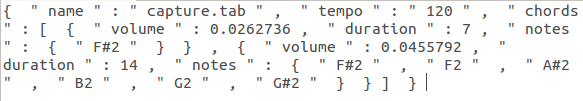
\includegraphics[scale=0.5]{FichierPartition}
\caption{Fichier representant une partition}
\end{figure}


\paragraph{}
Une grande amélioration serait également de rajouter la possibilité d'enregistrer plusieurs pistes. Cela permettrait donc de 
composer des musiques plus complètes avec par exemple une guitare rythmique et une guitare solo.

\paragraph{}
Les données de connexion à la base de données sont enregistrées en clair dans un fichier de configuration, il faudrait changer 
ce fichier et le crypté pour que les utilisateurs ne puissent pas accéder à cette donnée confidentielle.
